\chapter{Probing Lightning channel balances}

\label{Chapter06LNprobing}

The LN protocol provides no method for a node to query the distribution of funds in remote channels.
In this Chapter, we show that this information may not be private in practice.\footnote{This Chapter is based on~\cite{Tikhomirov2020}.}
We demonstrate how a low-resource attacker can infer balances of most channels by sending a fake payment (a \textit{probe}) and observing the resulting error.
Our \textit{probing} method shows better accuracy and cost compared to similar approaches described in the literature and scales to the whole network.
Compared to earlier approaches~\cite{HerreraJoancomarti2019, Dam2019}, we do not need to establish a channel with one of the endpoints of each target channel.
The ability to probe remote channels dramatically reduces the time and capital required for the attack.
Half of the channels can be probed in under $21$~seconds each.
The attacker does not spend the committed capital but only temporarily locks it up.
We test our proof-of-concept implementation on the Bitcoin testnet and successfully probe a significant portion of its channels.
We also outline potential countermeasures, including changes in error handling, sharing channel balances explicitly, and \textit{just-in-time} (JIT) routing.

On a more general note, we raise a question of the \textit{privacy-efficiency trade-off} in the LN\@.
On the one hand, the lack of information about channel balances increases the payment failure rate.
On the other hand, the LN does a poor job of protecting this information.
Can we strike a better balance between balance privacy and routing efficiency?
Answering this question remains an exciting avenue for future work.


\section{Probing algorithm}
\label{sec:probing}

\subsection{Overview}

As described in Chapter~\ref{Chapter05IntroLightning}, an LN channel operates as follows.
Two parties lock funds in a multi-signature UTXO and then change the distribution of funds in a sequence of off-chain payments.
Nodes gossip about channels available for routing and their total capacities.
To issue a multi-hop payment, the sender chooses a route based on its local knowledge of the network.
Nodes do not announce the distribution of funds in their channels.

Consider two adjacent LN nodes.
Let us denote the total capacity of their channel as $c$.
Without loss of generality, let us denote one of the nodes as \textit{source} (with balance $b_s$) and the other as \textit{destination} (with balance $b_d$).\footnote{The BOLT specification defines the source as the node with an alphanumerically smaller node ID.}
By definition, $c = b_s + b_d$.
Our goal is to determine how $c$~is split between $b_s$~and~$b_d$.
For concreteness, for each channel, we estimate $b_s$, and refer to it as $b$.

In a nutshell, our algorithm consists of the following steps:
\begin{itemize}
	\item set up a Lightning node;
	\item open a few \textit{entry channels} to manually selected nodes (\textit{entry nodes});
	\item compile a list of target channels;
	\item for each channel in the list, perform a binary search for the value of~$b$~by sending fake payments through routes ending with the target channel.
\end{itemize}

\subsection{Assumptions}

To be suitable for probing, the channel must be \textit{active} (available for routing) and \textit{live} (responding to requests).
We assume that nodes follow the BOLT specification (in particular, they return errors as prescribed).

\paragraph{Error interpretation}
We use two types of errors, which have a broader semantics than our method is aware of.
A node returns a \texttt{temporary\_channel\_failure} (\texttt{UPDATE|7}) error is it "was unable to handle this HTLC, but may be able to handle it, or others, later."
We interpret this error as "insufficient balance," though there may be other reasons for temporary channel unavailability.
A node returns \texttt{incorrect\_or\_unknown\_payment\_details} (\texttt{PERM|15}) if "[t]he payment\_hash is unknown to the final node, the payment\_secret doesn't match the payment\_hash, the amount for that payment\_hash is incorrect or the CLTV expiry of the HTLC is too close to the current block height for safe handling".
We interpret this error as only the first of the listed conditions.
The payment hash is unknown to the receiving node, as we generated it randomly.
Other conditions should not hold: the amount and the HTLC expiry date should be consistent, as we rely on the standard functionality of c-lightning to construct payments.
We assume it to be compliant with the specification and well-tested.
Experiments on our own channels showed that c-lightning indeed returns these errors under the conditions relevant to our experiment.

\paragraph{A note on probing directions}
Our probing algorithm is agnostic to the direction of probing payments.
For instance, sending a probe via a route ending in "Alice -- Bob" theoretically gives the same information as a probe via a route ending in "Bob -- Alice."
However, channel directions may have different properties in practice.
Each channel party controls the routing policy in its channel direction.
Alice may allow routing to Bob without Bob allowing routing to Alice.
To extract the maximum amount of information, we probe channels in both directions.
Doing so also helps us overcome the technical issue with large channels.
Due to the limitation on the LN payment amount, we cannot probe large channels.
However, if a large channel's capacity is skewed, we can successfully probe it from the "smaller" instead of the "larger" end.
For clarity, we omit this implementation detail from the algorithm description.

\paragraph{A note on applicability}
Our experiments demonstrate the probing technique's feasibility, but the results from the testnet cannot be directly applied to the mainnet.
In particular, the mainnet LN contains four times more channels than the testnet LN\@.
Therefore, probing the whole LN on the mainnet would take more than two~days instead of~$14$~hours.
We note that the attacker can still target specific channels, such as those belonging to an individual service provider.
Tens or hundreds of chosen channels can be probed in a feasible amount of time.
Probing selected channels would give the attacker valuable insights into the victim's financial situation.


\subsection{Selecting channels for probing}

First, we compile a list of active and live channels.
We define a channel as \textit{active} if at least one of its two directions is announced as active (available for routing) in the gossip data.
To determine liveness, we use the heuristics presented in Algorithm~\ref{alg:select-channels}.

\begin{algorithm}
	\KwData{Gossip data}
	\KwResult{Channels selected for probing}
	\For{node in gossip data} {
		connect to node\;
		\If{connection established}{add node to live nodes\;}
	}
	\For{channel in gossip data}{
		\If{source and destination in live nodes}{
			add channel to channels to probe\;
		}
	}
	\For{channel in gossip data} {
		send a $1\,000$~sat probe\;
		\If{error returned}{add channel to channels to probe\;}
	}
	\caption{Selecting channels for probing.}
	\label{alg:select-channels}
\end{algorithm}

\paragraph{Heuristic 1: Connecting to nodes}
For a channel to be live, both its parties must be live.
We extract a list of nodes from gossip data and establish a P2P connection to each of them.\footnote{Establishing a P2P connection is nearly instant and, unlike opening a channel, does not require capital commitment.}
We consider a channel live if both its parties are live.
We close all the connections after this step, except for the connections to our entry nodes.

\paragraph{Heuristic 2: Pre-probing}
To further optimize probing, we introduce a pre-probing step.
We send a probe of~$1\,000$~satoshis to every channel marked as active in the gossip data\footnote{We use the same probing function as for the main probing.}.
If we get no response, we consider the channel dead and do not consider it in the main probing step.
For the first round of probing, we consider all channels classified as live by either the first or the second heuristic.

\paragraph{Heuristic 3: Liveness detected during probing}
Each probe results in an error propagated back to the sender.
During the first probing round, we expand our list of live channels.
If we issue a probe along the route of channels $c_1, c_2, \dots, c_n$~and receive an error from channel $c_i$, we conclude that all preceding channels $c_j, j<=i$~are live.
If any of~$c_j$~is not on our live channels list, we add it.
During the second probing round, we use the updated live channels list.


\subsubsection*{Channel order}
We say that channel $c_1$~is \textit{closer} to us than channel $c_2$, if the shortest route from our node to one of the endpoints of~$c_1$~is shorter than that for $c_2$.
We informally refer to a channel as \textit{important}, if a large share of our probes is forwarded through it.
Our method is agnostic to the order in which we probe the channels.
However, we choose to probe the "closer" and more "important" channels first.
The rationale is that it is beneficial to first probe the channels often used as intermediary hops.
Knowing their balances allows us to avoid sending payments that would fail due to insufficient balance at an intermediary hop.

We probe channels in the following order:

\begin{enumerate}
	\item channels adjacent to our entry nodes (the "first layer");
	\item channels between hubs -- channels connecting nodes out of~$1\%$~of the most connected nodes (if not already probed);
	\item channels adjacent to the "first layer" (if not already probed);
	\item all other channels (if not already probed).
\end{enumerate}

\subsection{Probing}

After compiling a list of live and active channels, we issue a series of probes to each of them.

Recall that in the ordinary course of operation, the payment receiver generates a random value $r$~and sends its hash $h = H(r)$ to the sender.
The sender then creates a series of HTLCs with the same hash value $h$.
A probe is an unsolicited payment with a random value instead of~$h$.
Such payments fail in any case.
However, we can obtain the information on channel balances based on which error occurred and where.
In particular, we can infer whether the balance of the erring channel is higher than the probing amount $a$.
Intermediary nodes cannot distinguish randomly generated and genuine payment hashes.
They will, therefore, forward our probes as regular payments.
If all channels along a route have sufficient balances (higher than $a$), the probe only fails at the last step.
The final recipient finds out that it does not know the preimage for the payment hash and emits the corresponding error message.
If any channel along the route has insufficient capacity, the payment fails at that channel before reaching the final recipient.

Let $c_1, c_2, \dots, c_n$~be a sequence of channels in a route, and~$b_i$~be their respective balances.
Let $c_j$~be the erring channel.
After each probe with an amount $a$, we obtain the following information:
\begin{itemize}
	\item $b_i > a$~for $i<j$;
	\item $b_j < a$~if the error is "insufficient capacity", or $b_j > a$~if the error is "unknown preimage".\footnote{The latter is only possible if $j=n$.}
\end{itemize}

The probing algorithm for a single route is presented in Algorithm~\ref{alg:probe-route}.

\begin{algorithm}
	\KwData{Route and amount to probe}
	\KwResult{Updated balance estimates for channels in route}
	send payment along route\;
	\For{channels before erring channel} {
		$b_{min} = a$\;
	}
	\For{erring channel}{
		\If{insufficient funds}{
			$b_{max} = a$\;
		}
		\If{unknown preimage}{
			$b_{min} = a$\;
		}
	}
	\caption{Probing a route.}
	\label{alg:probe-route}
\end{algorithm}

For each channel, we keep a lower ($b_{min}$) and an upper ($b_{max}$) bound for its balance $b$.
Initially, $b_{min}=0$~and~$b_{max}=c$.
At each probing step, we aim at shrinking this interval with binary search, i.e.,~by issuing a probe with the amount of~$\frac{1}{2} (b_{min} + b_{max})$.
If the midpoint between $b_{min}$~and~$b_{max}$~is larger than the maximum HTLC amount allowed by the specification, we decrease it to that maximum minus a safety margin.
The algorithm for all channels selected for probing is presented in Algorithm~\ref{alg:probe-channels}.

\begin{algorithm}
	\KwData{Gossip data}
	\KwResult{Improved estimates for channels}
	SelectChannelsForProbing\;
	\For{channel in channels for probing} {	
		$b_{min} = 0$\;
		$b_{max} = c$\;
		\For{number of probings per channel} {
			\For{number of attempts per probing}{
				GetRouteToTargetChannel\;
				ProbeRoute\;
				\For{channel in route}{
					\If{channel is live and not marked as live}{
						mark channel as live
					}
				}
				\If{target channel estimates updated}{
					continue\;
				}
			}
			\If{required precision reached}{
				continue\;
			}
		}
	}
	\caption{Probing all channels.}
	\label{alg:probe-channels}
\end{algorithm}


\paragraph{Choosing routes}

For each probe for a chosen \textit{target channel}, we select routes towards it based on the following criteria:
\begin{itemize}
	\item the target channel is the last channel in the route;
	\item all previous channels in the route have sufficient balances (to the best of our current knowledge) to forward the probe.
\end{itemize}

The route generation algorithm is presented in Algorithm~\ref{alg:find-route}.

\begin{algorithm}
	\KwData{target channel, amount $a$}
	\KwResult{Route to target suitable for $a$}
	\For{channels adjacent to destination} {
		\If{channel is not target}{
			add channel to excluded channels\;
		}
	}
	\For{all channels}{
		\If{$a > c_{max}$}{
			add channel to excluded channels\;
		}
	}
	\While{route is bad}{
		get route to target without excluded channels\;
		\For{channel in route}{
			\If{$a > b_{max}$}{
				route is bad\;
			}
		}
		route is good\;
	}
	\Return route\;
	\caption{Getting a route to the target channel.}
	\label{alg:find-route}
\end{algorithm}

We rely on the built-in functionality of our LN node (c-lightning) to generate routes.\footnote{Internally, c-lightning uses the Dijkstra algorithm.}
The c-lightning API allows us to customize routes, excluding specified nodes and channels.
We use this functionality to pre-filter suggested routes based on the information we have obtained through probing so far.
If we know that a balance of some channel in a suggested route is insufficient, we exclude this channel from consideration for the current probe.
This filtering allows us to speed up the probing by not sending probes through routes with insufficient balances in intermediary channels.

Finally, we perform the second probing pass to probe the channels that have been only detected as live during the first pass (the third liveness heuristic).

\paragraph{Channel information coefficient}
To measure the effectiveness of our technique, we introduce the \textit{channel information coefficient}.
Let $c$~is the original channel capacity, and~$b_{max}$~and~$b_{min}$~be our upper and lower bound estimates for $b$.
Then the information coefficient is defined as:

\[i = 1 - \frac{b_{max} - b_{min}}{c}\]

Thus, $i = 0$~means that we do not know any extra information about $b$~besides public knowledge.
The value $i = 1$~means that we know $b$~precisely.


\section{Experimental setup}

We implement the algorithm described in~\cref{sec:probing} as a c-lightning plugin.
The plugin functionality allows developers to integrate Python code with the c-lightning node~\cite{clightningPlugins}.
We only collect data from the Bitcoin testnet.
We try to perform at least $7$~probings per channel, which means that in a successful probing, we shrink the $[b_{min}, b_{max}]$~interval to $\frac{1}{128}$~of its initial length, determining $b$~with the precision better than $1\%$.

\paragraph{Entry nodes}
We launch our own LN node\footnote{c-lightning version \texttt{v0.8.0-40-g899f5de}.} and fund it with testnet coins.
Then, we establish five~entry channels to handpicked nodes with high connectivity and liquidity.
Four of our channels have the maximum standard capacity of~$0.167$~BTC\@.\footnote{LN limits the channel capacity at $0.167$~BTC\@. Larger channels can be created with a special command-line argument and are sometimes called \textit{wumbo channels}.}
One entry channel has a capacity of~$0.043$~BTC\@.
We choose nodes to connect to based on the following requirements (as reported by 1ML~\cite{1MLTopConnected}):
\begin{itemize}
	\item well-connected and well-capitalized;
	\item located relatively close to our node (i.e.,~in Europe) to decrease latency.
\end{itemize}

\paragraph{Choosing the timeout}
One of the decisions we have to make is to set a timeout, after which we declare a channel unresponsive and move to the next one.
The LN protocol does not prescribe how quickly a node should react.
The only time limitation is the HTLC timeout, usually on the order of hours or days.
Therefore, to probe all channels in a reasonable time, we choose a timeout of~$10$~seconds.
Our later results showed that this was a reasonable trade-off between probing speed and accuracy.

\paragraph{Route selection}
We generate routes with the standard c-lightning \texttt{getroute} routine and exclude routes with known insufficient balances in intermediary channels.
Note that route generation is a local operation.
One route generation takes under $10$~ms in our experiments, two orders of magnitude less than the average probe response time ($3$~seconds).

In our main experiment, we perform $12\,895$~payments.
We reject $96\,768$~routes because of low balance.
That is, we filter out around $8$~routes per payment.
Therefore, our method of route generation does not significantly increase the time of our experiment.
This approach may be improved with custom route generation.

Another trade-off we have to address is the maximum route length.
The LN protocol limits the length of a route to $20$~channels.
Longer routes allow collecting more information per probe but increase the probability of failure at intermediary channels.
For our experiment, we limit the length of routes to $10$~channels.

\paragraph{Hanging HTLCs}
Our method assumes that an error is returned quickly (within seconds, as Figure~\ref{fig:route-length-timings} shows).
If some intermediary hop does not return an error, our entry channels are left with an unresolved in-flight HTLC that we call \textit{hanging}.
Hanging HTLCs occupy our channels' capacity, preventing us from issuing large probes from the affected channel.
The protocol does not allow canceling HTLCs unilaterally, and closing a channel involves long timeouts until the funds are available and can be committed to a new channel.
Therefore, we use multiple entry channels to be able to tolerate some hanging HTLCs.
This issue is related to the attack presented in Chapter~\ref{Chapter08HTLClimit} and the one described in~\cite{Mizrahi2020}.

\section{Results} \label{sec:results}

The LN on the Bitcoin~testnet contains $1\,974$~nodes and~$5\,884$~channels, including $2\,527$~announced as active (as of 26~February~2020).
The initial estimate shows that $207$~nodes and~$1\,625$~channels are live.
We detect $3$~more live channels during the first probing pass.
The strongly connected component of the live subgraph contains $1\,489$~channels.
The other $139$~channels point towards nodes for which we could not get meaningful error messages.

We send $3\,153$~($24.45\%$) during the pre-probing and $9\,742$~($75.55\%$) during the main probing phase ($12\,895$~probes in total).
Out of~$9\,742$~probes in the main phase, $8\,256$~($84.75\%$) return errors that we can use to improve the balance estimates ("channel temporary unavailable" and "incorrect or unknown payment details").
The time of the experiment is~$14$~hours and~$6$~minutes.
Probing $1\,628$~live channels takes $65\%$~of the time (roughly $9$~hours).
The rest is spent on slow-responding channels or channels that reply with an unexpected error.


\subsection{Probing times}

First, we consider the distribution of probing times for various route lengths (Figure~\ref{fig:route-length-timings}).

\begin{figure}[ht]
	\centering
	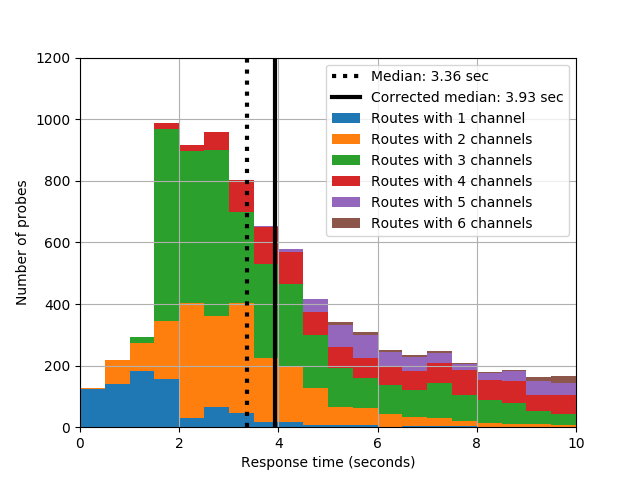
\includegraphics[width=0.8\textwidth]{route-length-timings.png}
	\caption{The distribution of probes (onions) by response time.}
	\label{fig:route-length-timings}
\end{figure}

Nearly all probes sent along the routes of $3$~hops and shorter return within $10$~seconds.
The median of the $8\,256$~probes is at $3.36$~seconds.
Recall that $15.25\%$~of the probes time out or return an error that we cannot interpret within our algorithm.
The corrected median without the timed out and erring probes is $3.93$~seconds. 
We conclude that the cutoff at $10$~seconds presents an acceptable trade-off.
The diameter of the strongly connected component on the LN is~$3$.\footnote{It is not always possible to use the shortest route, as it may not have sufficient balances in all channels.}

Next, we consider the time it takes to probe a single channel.
With the parameters we have chosen, each probe cannot take longer than $70$~seconds ($7$~probes of up to $10$~seconds each).
For each channel, we add up the times of probes sent to this channel.
Figure~\ref{fig:channel-timings-CDF} shows the cumulative distribution function of channels by the total time spent probing them.
We observe that $50\%$~of channels can be probed in less than $21.2$~seconds.

\begin{figure}[ht]
	\centering
	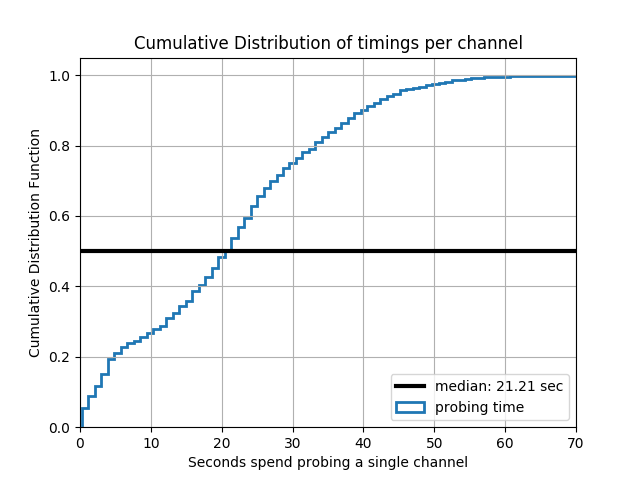
\includegraphics[width=0.8\textwidth]{channel-timings-CDF.png}
	\caption{Distribution of channels by total probing time.}
	\label{fig:channel-timings-CDF}
\end{figure}


\subsection{Probing coefficients}

We use the channel information coefficient to measure how much information we obtain for each channel.
The LN specification limits the value of a single payment to $0.043$~BTC\@.
We denote channels with the capacity more than two times that (i.e.,~$2 \times 0.043 = 0.086$~BTC) as \textit{large channels}.
We call other channels \textit{small}.
All small channels can, in principle, be fully probed.
A large channel can only be fully probed if the local balance at one of its endpoints is smaller than the maximum payment amount.

\begin{figure}[ht]
	\centering
	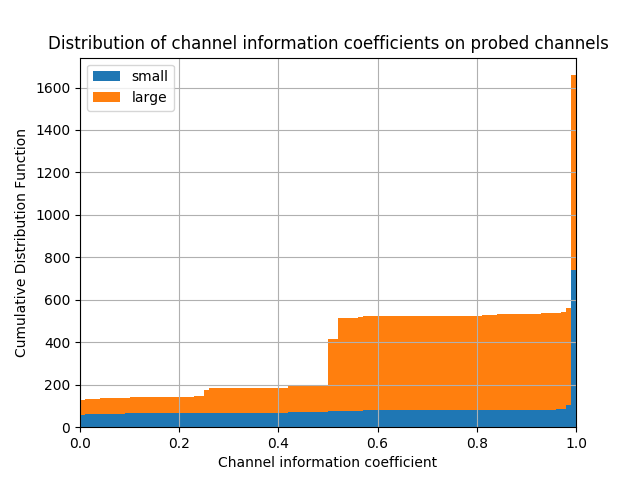
\includegraphics[width=0.8\textwidth]{cdf-channel-coefficients.png}
	\caption{Distribution of channels by the obtained information coefficient.}
	\label{fig:cdf-channel-coefficients}
\end{figure}

Figure~\ref{fig:cdf-channel-coefficients} represents the distribution of channels by their information coefficients.
We obtained full balance information on over $1\,000$ of~$1\,628$~channels.
We explain the jump at $0.5$~for the large channels as follows.
The maximum standard channel capacity ($0.167$~BTC) is approximately four times the maximum HTLC amount ($0.043$).
Consider a channel with a total capacity of~$0.167$~BTC and the local balance between $0.043$~BTC and~$0.167 - 0.043 = 0.124$~BTC\@.
We probe this channel from both sides and receive the "unknown hash" error in both cases.
From that, we conclude that the local balance is between $0.043$~BTC and~$0.124$~BTC\@.
This estimate yields a channel information coefficient of~$0.515$.
However, with our current technique, we cannot improve it.

\subsection{Distribution of channels in routes}

We also want to understand how often we send probes through each channel.
Most of our routes go through the same few channels (Figure~\ref{fig:channel-frequency-distribution}), which is partially explained by the fact that all routes include one of our entry channels.

\begin{figure}[h]
	\centering
	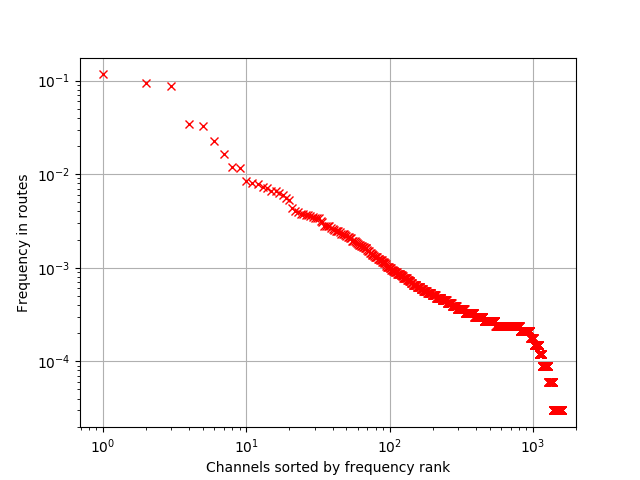
\includegraphics[width=0.8\textwidth]{channel-frequency-distribution.png}
	\caption{Distribution of relative frequencies of channels in routes.}
	\label{fig:channel-frequency-distribution}
\end{figure}


\subsection{How balanced are the channels?}

A channel is informally called \textit{balanced} if the parties have roughly equal balances.
We introduce the \textit{balance coefficient} to quantify this.
The balance coefficient represents the distance from the actual channel balance to $0.5$~of the total capacity, where $b$~is the estimated local balance and~$c$~is the total channel capacity:

\[c_{bal} = 0.5 - \frac{|b-c|}{c} \]

A channel is unbalanced if its whole capacity is on one side ($c_{bal} = 0$).
A channel is perfectly balanced if the two parties have equal balances ($c_{bal} = 1$).

\begin{figure}[h]
	\centering
	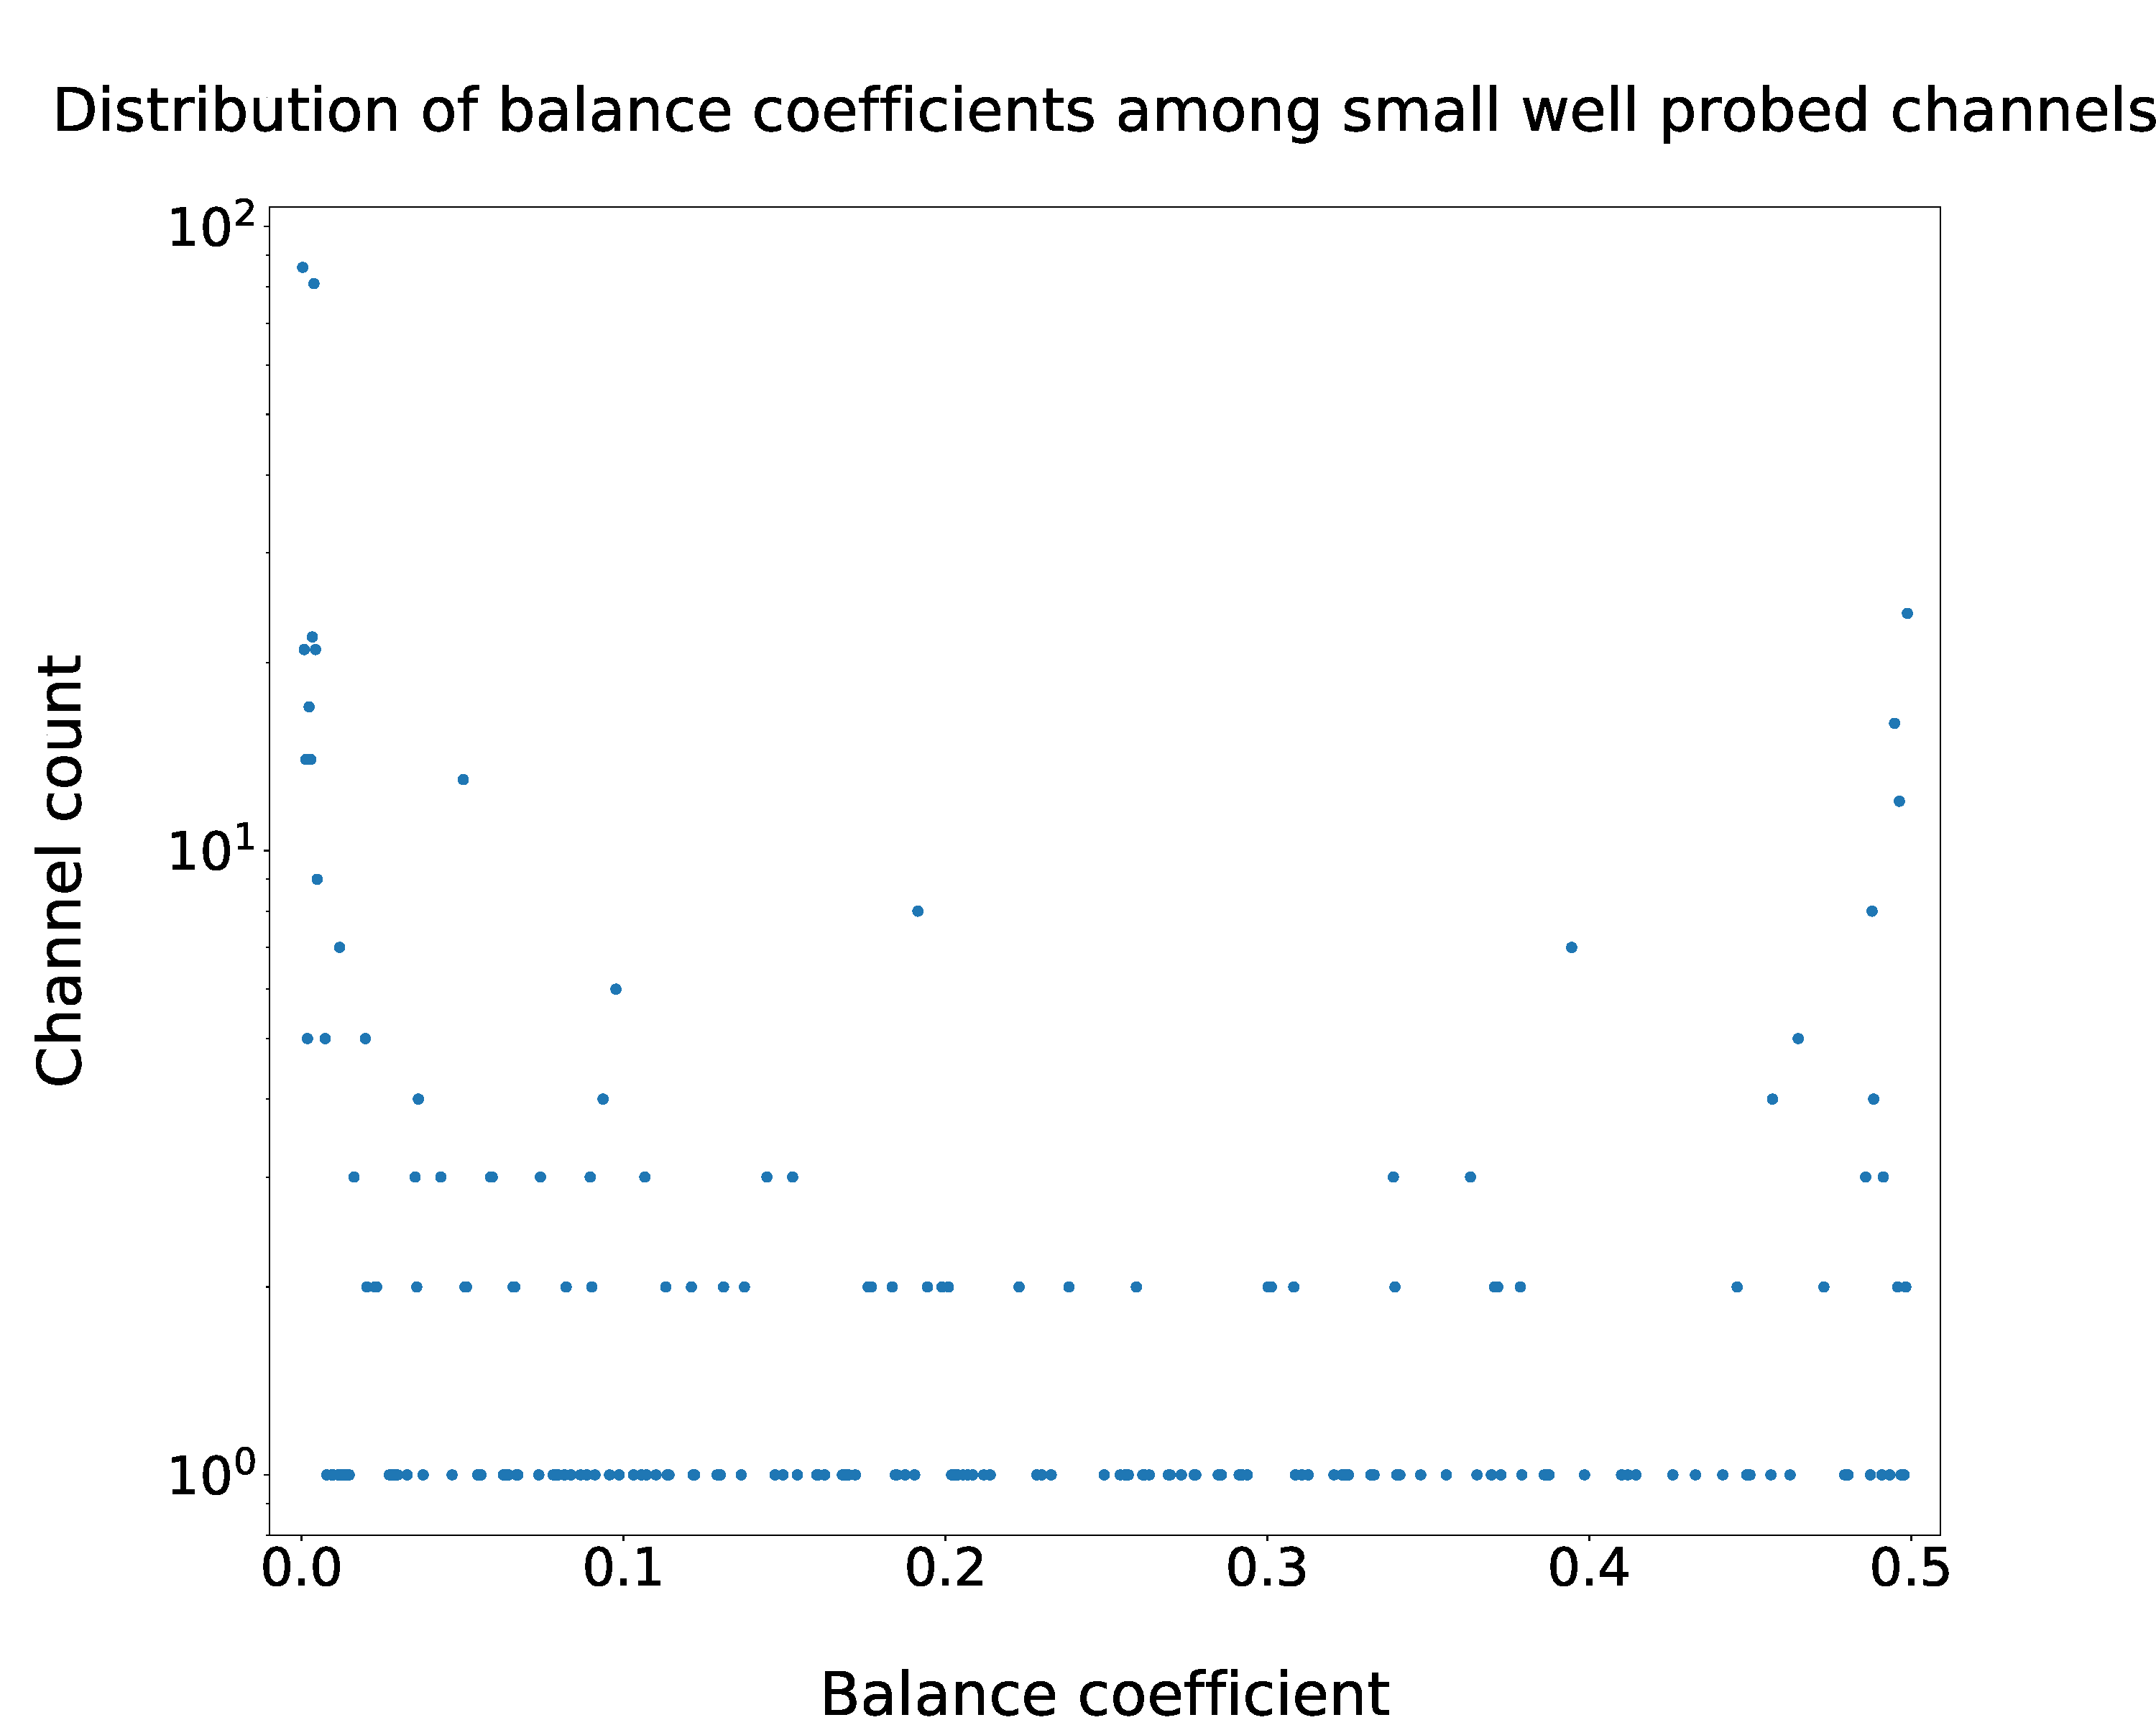
\includegraphics[width=0.8\textwidth]{balance-coeff-histogram.pdf}
	\caption{Distribution of balance coefficients.}
	\label{fig:balance-coeff-histogram}
\end{figure}

Figure~\ref{fig:balance-coeff-histogram} depicts the distribution of balance coefficients among "small" channels that we are able to probe with high accuracy (information coefficient higher than $0.9$).
We conclude that many small channels are unbalanced (coefficient close to zero).
$15\%$~have the balance coefficient below $0.001$, $45\%$~below $0.01$, and~$62\%$~below $0.1$.
However, note that the picture may change if we consider large channels, and that channel management practices on mainnet may differ.


\section{Estimating the attack cost}

The attack requires moderate resources.
The attacker only needs to commit funds to the entry channels.
The capacities of the entry channels determine the maximum probing amount.
The computational and communication requirements are similar to the ones required to run a standard LN node.
The adversary only needs to maintain a few TCP connections during the main phase of the experiment.
(We also open and immediately close connections to all nodes to check their liveness; this process can be parallelized.)
Note that running an LN node implies running a fully synchronized Bitcoin node, which requires hundreds of gigabytes of storage ($265$~GB at the time of our experiments in February~2020).

With our current approach, the maximum probing amount is the protocol's HTLC limit of~$0.167$~BTC\@.
This is the minimal amount the attacker has to commit to theoretically be able to probe all "small" channels fully.
Our experience shows that it is beneficial to open multiple channels to decrease the negative effect of hanging HTLCs.
In our experiments, we use five~entry channels.

Note that since all the probing payments fail, the attacker pays no fees.
If no HLTCs are left unresolved after the probing, the attacker can close the entry channels collaboratively and withdraw the committed funds immediately.
If some HTLCs are left unresolved, or the attacker's channel partners are offline or unwilling to cooperate on channel closure, the attacker would have to wait for the agreed-upon timeout (usually on the order of days) before withdrawing the funds.
In any case, no coins are irrevocably lost.
However, the attacker still bears the opportunity cost: the coins committed to the attack could have been invested elsewhere.

\pagebreak

\section{Limitations}

Now we discuss the limitations of our approach and potential ways to improve it.

\paragraph{Private channels}

LN nodes do not have ao announce their channels.
For example, casual users using mobile devices are not supposed to do so
According to a 2020 study~\cite{BitMEXPrivateChannels}, $28\%$~of LN~channels are unannounced.\footnote{Unannounced channels are also called \textit{private}.}
Unannounced channels are not prone to our probing methodology.
The sender does not know the private channel endpoint's identifier and cannot construct a route to it.

It may be possible to extend our technique with on-chain heuristics to locate unannounced channels.
In particular, each channel has a short identifier composed of the block number, the transaction index, and the UTXO index of the funding transaction's multisignature output.
An attacker may scan the blockchain looking for such outputs and cross-reference them with the LN gossip data~\cite{Pickhardt2020}.

\paragraph{Lack of suitable routes}

We cannot probe a route if we do not find a suitable route to the target channel.
In particular, we cannot probe a high-capacity channel if only a low-capacity channel connects it to the rest of the network.
We can partially overcome this limitation by diverging from the series of probing amounts determined by binary search.
Recall that for each yet unknown channel balance $b$~we maintain the current estimation interval $[b_{min}, b_{max}]$.
The binary search prescribed to choose the next probing amount as $\frac{b_{min} + b_{max}}{2}$.
If this value is too high, we may instead use the maximum value for which we can find a suitable route.
Decreasing the probing amount would allow us to obtain at least some information on the channel in question.
In the initial version of our algorithm, we do not do it for simplicity.

\paragraph{Concurrent probing of large channels}

Recall that our method cannot fully probe large channels because of the limitation on the HTLC amount.
Lightning implementations impose a limit on the maximal amount transferred in one HTLC\@.
This limit is approximately $0.043$~BTC\footnote{4294967295 millisatoshis.}.
Therefore, we can only fully probe channels where the local balance of one of the channel parties is below $0.043$~BTC\@.

A possible way to overcome this limitation would be to probe large channels with multiple HTLCs concurrently.
The goal of concurrent probing is to temporarily block the capacity of the attacked channel.
Our current method does not allow concurrent probing because we only control the sender, not the receiver.
An honest receiver quickly returns an error and unblocks the capacity.
Concurrent probing would involve a malicious node acting as the receiver of all our probes.
The malicious receiver would deliberately delay the response, thus temporarily blocking funds along the route.

Concurrent probing could also decrease the probing time, bringing the results closer to an instant network snapshot.
However, adding concurrency is a non-trivial task.
Parallel probings may interfere with each other if the same channel is involved in two routes probed simultaneously.

Note also that some realistic attack scenarios do not involve probing the whole network.
An adversary may choose one "important" Lightning node and probe all its channels relatively quickly.
The obtained information may be a business secret of the node operator.

\paragraph{Parallel channels and non-strict forwarding}

Our method is based on the assumption that the probe is forwarded through the \textit{channels} determined by the sender.
However, the LN specification only guarantees that the payment follows the chosen sequence of \textit{nodes}.
A pair of nodes may share multiple channels (\textit{parallel channels}).
A forwarding node is free to choose a channel from all parallel channels to the next node.
This practice is known as \textit{non-strict forwarding} and provides flexibility in addressing local balance restrictions.
While the LN specification allows non-strict forwarding, c-lightning does not allow opening multiple channels to the same node.
The other two popular implementations, LND and Eclair, support parallel channels.
Therefore, we cannot ensure that an intermediary node uses a given channel.
It may forward out probe through a parallel channel instead.
We accept this issue as a limitation of our approach.

As seen from our LN snapshot dated 25~February~2020, the mainnet LN contained $1\,438$~parallel channels ($17.64\%$~of all channels), which indicates that the effects on the probing precision could be significant on mainnet\footnote{Unannounced parallel channels may also influence our results.}.
However, most \textit{node pairs} have at most one channel, which thus can be probed using our method.


\section{Countermeasures}

The simplest countermeasure that does not require protocol changes can be implemented as part of a node routing policy.
Note that all our probing payments fail (either due to insufficient balance or unknown hash preimage). 
Intermediary nodes know whether a payment they are a part of succeeds or fails.
Therefore, an intermediary node observing a flood of failing payments from the same channel may suspect a probing, especially if the amounts follow the binary search pattern.
An intermediary node can then close the channel or otherwise limit the flow of failing payments from the node in question.
Of course, the adversary can trick such detection techniques, for example, by connecting to Bob via Alice and making Bob think that Alice is performing the probing.

We divide the other potential countermeasures into two categories: prioritizing privacy and prioritizing efficiency.


\subsubsection*{Prioritizing privacy}

We argue that reliably protecting channel balances in the LN is currently infeasible.
This conclusion comes from the following observations:
\begin{itemize}
	\item the sender knows whether the payment has failed or succeeded;
	\item if the payment fails, the sender knows the erring channel.
\end{itemize}
However, we can change the protocol to make the latter assumption not hold.

\paragraph{Merging error types}
When a payment fails, the sender receives an error message.
Depending on the cause of the error, these messages differ in two ways.
They have different error codes and originate from different nodes.
In particular, if the target channel has insufficient balance, the error is returned by the \textit{previous} node.
If the target channel has enough balance, then the \textit{final recipient} reports incorrect payment details.
We propose a change to error handling in the LN that would prevent the sender from knowing where the payment has failed.
In particular, each node in a route changes the error it sends back as if it has originated from its own channel.
We also suggest merging the two error types ("incorrect or unknown payment details" and "temporary channel failure").
A similar countermeasure has already been implemented (see note about error types $16$~and~$17$~in BOLT4~\cite{Bolt4OnionRouting}).
The drawback of this method is a decrease in payment reliability.
The sender can no longer exclude the failing channel from the subsequent route search.
However, the payment reliability problem may become less pressing with \textit{multi-part payments} (MPP) that split a large payment into small parts and thus increase routing efficiency.

\paragraph{Added loops}
Another potential countermeasure would be for intermediary nodes to add extra hops to the route.
Currently, the sender chooses the route.
The order of nodes in the route is enforced with onion routing.
If this scheme is modified, an intermediary node could instead forward the payment to the next node in the route through an added random sub-route.
Added loops would blur the picture for the sender, as the sender would not know which path the payment has taken.
One drawback of this approach is the requirement to substantially change the onion routing protocol, which, as~\cite{Malavolta2019} argues, is necessary for LN security.
The fee structure would also have to be more complex.

\paragraph{JIT routing}
Just In Time Routing (JIT routing) algorithm ha been originally proposed to improve payment reliability~\cite{Pickhardt2019, Pickhardt2019a}.
JIT routing works as follows.
If a forwarding node lacks the balance to forward a payment, it sends a circular payment to itself to add more funds to the necessary channel.
This process is called \textit{channel rebalancing}.\footnote{Another research paper~\cite{Conoscenti2019} analyzes the influence of hubs on LN and proposed a channel rebalancing algorithm.}
A JIT-supporting node does not send an error message back if it lacks funds on the attacked (probed) channel in the probing scenario.
Instead, it interrupts the routing process, re-balances its channels, and then continues the forwarding.
The attacker would interpret the lack of error as a signal that the target channel has enough funds, but the same would hold if the channel is probed from the other side.
JIT routing can be an effective countermeasure against channel probing attacks.
However, timing attacks may become an issue.


\subsubsection*{Prioritizing efficiency: sharing balance data}

If hiding LN channel balances is infeasible, we may want to use balance information to improve routing efficiency.
Broadcasting all intermediate balances to all nodes would introduce a large networking overhead.
We propose to develop a reasonable method for nodes to share information about their channel balances selectively.
This information would improve path-finding and help nodes decide how to allocate funds to new channels.
We propose adding an API call that would allow the sender to query a channel's balance it wants to route a payment through.
In this scenario, a sender creates a preliminary route and asks the nodes along this route, whether they have sufficient balance.
If some of them do not, the sender re-calculates the route until a suitable route is found.
This algorithm would improve upon the current LN payment workflow, where a sender is receiving errors and re-sending a payment along multiple routes until it succeeds.
Nodes could develop policies regarding balances, for instance, only reveal balances to trusted nodes, or only to nodes that pay a fee.
A node's ability to reveal a channel balance for routing purposes may also be subject to negotiation between channel partners during channel establishment.
A detailed analysis of this protocol is needed to prevent abuse.


\section{Conclusion} \label{sec:conclusion}

Hiding balances from everyone except for the channel parties is a cornerstone of L2 privacy.
Making intermediate channel balances available would enable revealing remote channel balances in real time.
However, unknown local balances decrease routing efficiency.
The sender cannot know in advance whether the chosen route can handle the required amount.
Therefore, LN payments often fail due to insufficient balance at an intermediary hop.
In that case, the payment is attempted again with a different route.
The sender could prevent such failures if it knew the channel balances in advance.

Our experiments show that channel balances cannot be considered private data.
A low-resource attacker can probe the balances of most live and active channels with high precision.
We implement and evaluate our technique on the Bitcoin testnet, successfully probing a large portion of channels.
We identify a \textit{privacy-efficiency trade-off}: hidden balances improve privacy but hinder routing efficiency.
LN does not address this trade-off optimally: channel balances are neither well protected nor utilized.
We envision two paths for LN development with either privacy or routing efficiency prioritized.
Future research is needed to find the right balance between the two.
